\section{Experimental QPI measurement}
Real space \ac{QPI} signals are obtained by taking the grid map experiment on a region that presents \ac{QPI} patterns. In this section we will briefly explore \ac{QPI} measurement in the \ac{STM} experiment, more specifically, we will introduce the factors that dictates \ac{QPI} quality, discuss how to choose proper parameters that result in a good \ac{QPI} measurement, and finally we will present a specific challenge called the phase noise, which motivates our work in the next chapter.


\subsection{QPI measurement and quality}
As mentioned in Ch.2, taking a grid map is very involved. A successful grid map requires both an ideal instrumental setup, and a set of proper measurement parameters based on the understanding of the targeting material. 

The key objective of an ideal instrumental setup is to create a stable environment and lower the system noise, as we discussed in Ch.2, this involves minimizing the noise from mechanical vibration, temperature fluctuation, and electronic instability of the system, and maintaining a stable tip-surface tunneling junction. 

A grid map is defined by a $N\times N$ (assuming square) grid of on a targeted area of $L \times L$ $nm^2$, this provides a spatial resolution $\Delta L = \frac{L}{N}$; In reciprocal space, this set up gives a range $Q = \frac{2 \pi}{\Delta L}$ with resolution $\Delta Q = \frac{2\pi}{L}$, the energy range and resolution is defined by the setting of the single-point spectroscopy performed on every grid point. 

A set of proper parameters for \ac{QPI} measurement aims to extract the most amount of information with the highest level of resolution given the constrains of the system. The most important constrain is the limiting cryogenic holding time; This puts a ceiling to the grid map run time, while different system varies, typically the cryogenic holding time is a fraction of a week. Within the boundary of the run time, we usually aim for a grid with a fine reciprocal resolution $\Delta Q$ and a reasonable reciprocal range $Q$, corresponding to a large field of view $L$ and a reasonable $\Delta L$. It is intuitive to have a proper size of reciprocal range $Q$ that is not infinitely large, as most of the q-space features resides within the Bragg peaks, exemplified by Fig. \ref{fig:ch5_ldos} c). But we also do not want the field of view $L$ to be too large, this is because in real experiment with finite noise level, the featured \ac{QPI} pattern has a finite lifetime and its intensity will dive under the noise at some cutoff distance $r_{cutoff}$ from the defect center; Thus, a field of view larger than the cutoff distance will instead decrease the signal to noise ratio. We illustrate cutoff distances in systems with different noise levels in Fig. \ref{fig:ch5_cutoff}. The noise level is set to be noiseless, SNR = 10 and SNR = 1.2, respectively, given noise level shown in green dotted line, we identify the furthest signal peak higher than the noise level and place a blue vertical line there. These vertical lines indicate the cutoff distances; and we can see with increasing noise level, $r_{cutoff}$ drops, and thus the optimal field of view should also drop.  

\begin{figure}
	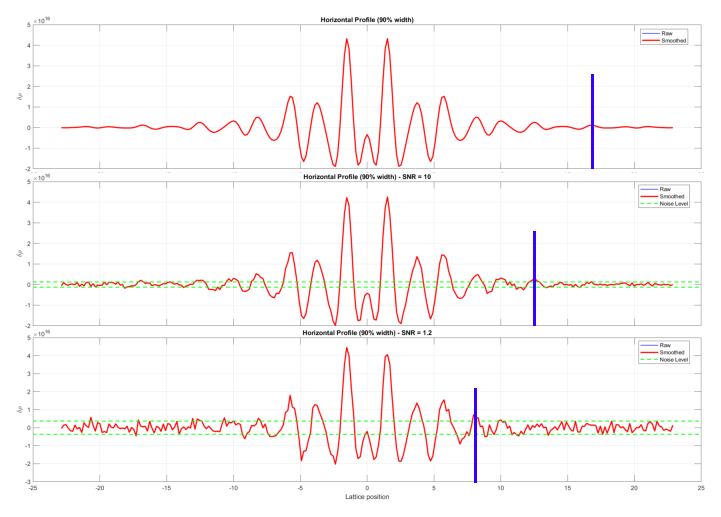
\includegraphics[width=\textwidth]{Ch5_fieldofview.pdf} 
	\centering
	\caption{Cutoff distances of QPI patterns with different signal to noise ratio. Three Horizontal Line profile on $\delta\rho(\textbf{x}, E=0.45eV)$ with noise of various levels. a) has no noise applied; b), c) have Gaussian noises applied with SNR = 10 and 1.2, respectively. Here the signal strength is defined as the variance of the noiseless $\delta\rho(\textbf{x}, E=0.45eV)$, see a) of Fig. \ref{fig:ch5_single_scattering}.}
	\label{fig:ch5_cutoff}
\end{figure}


\subsection{multi-defect QPI pattern and phase noise}
\ac{QPI} patterns present themselves around defects. While an ideal \ac{QPI} measurement is performed on an isolated defects in large field of view, it is normally difficult to find such a case. In real experiment, grid maps are usually taken on areas with multiple defects, this causes interference between the \ac{QPI} patterns originated from different defects, as hinted by Ch.5.2.4 when discussing Fig. \ref{fig:ch5_multi_scattering}.

This is problematic when we try to interpret the \textbf{q}-space \ac{QPI} map. As illustrated in Fig. \ref{fig:ch5_phasenoise}, when we have multiple defects scattered in the field of view, we start to see some noise patterns associated with the spatial distribution of the defects, as we can see by comparing c) and e), we see that with nothing but the relative locations of the defects changed, the corresponding \textbf{q}-space \ac{QPI} maps possess different noise patterns. This effect is called the phase noise, it hindered our ability to analyze the underlying quasiparticle scattering process. 

\begin{figure}
	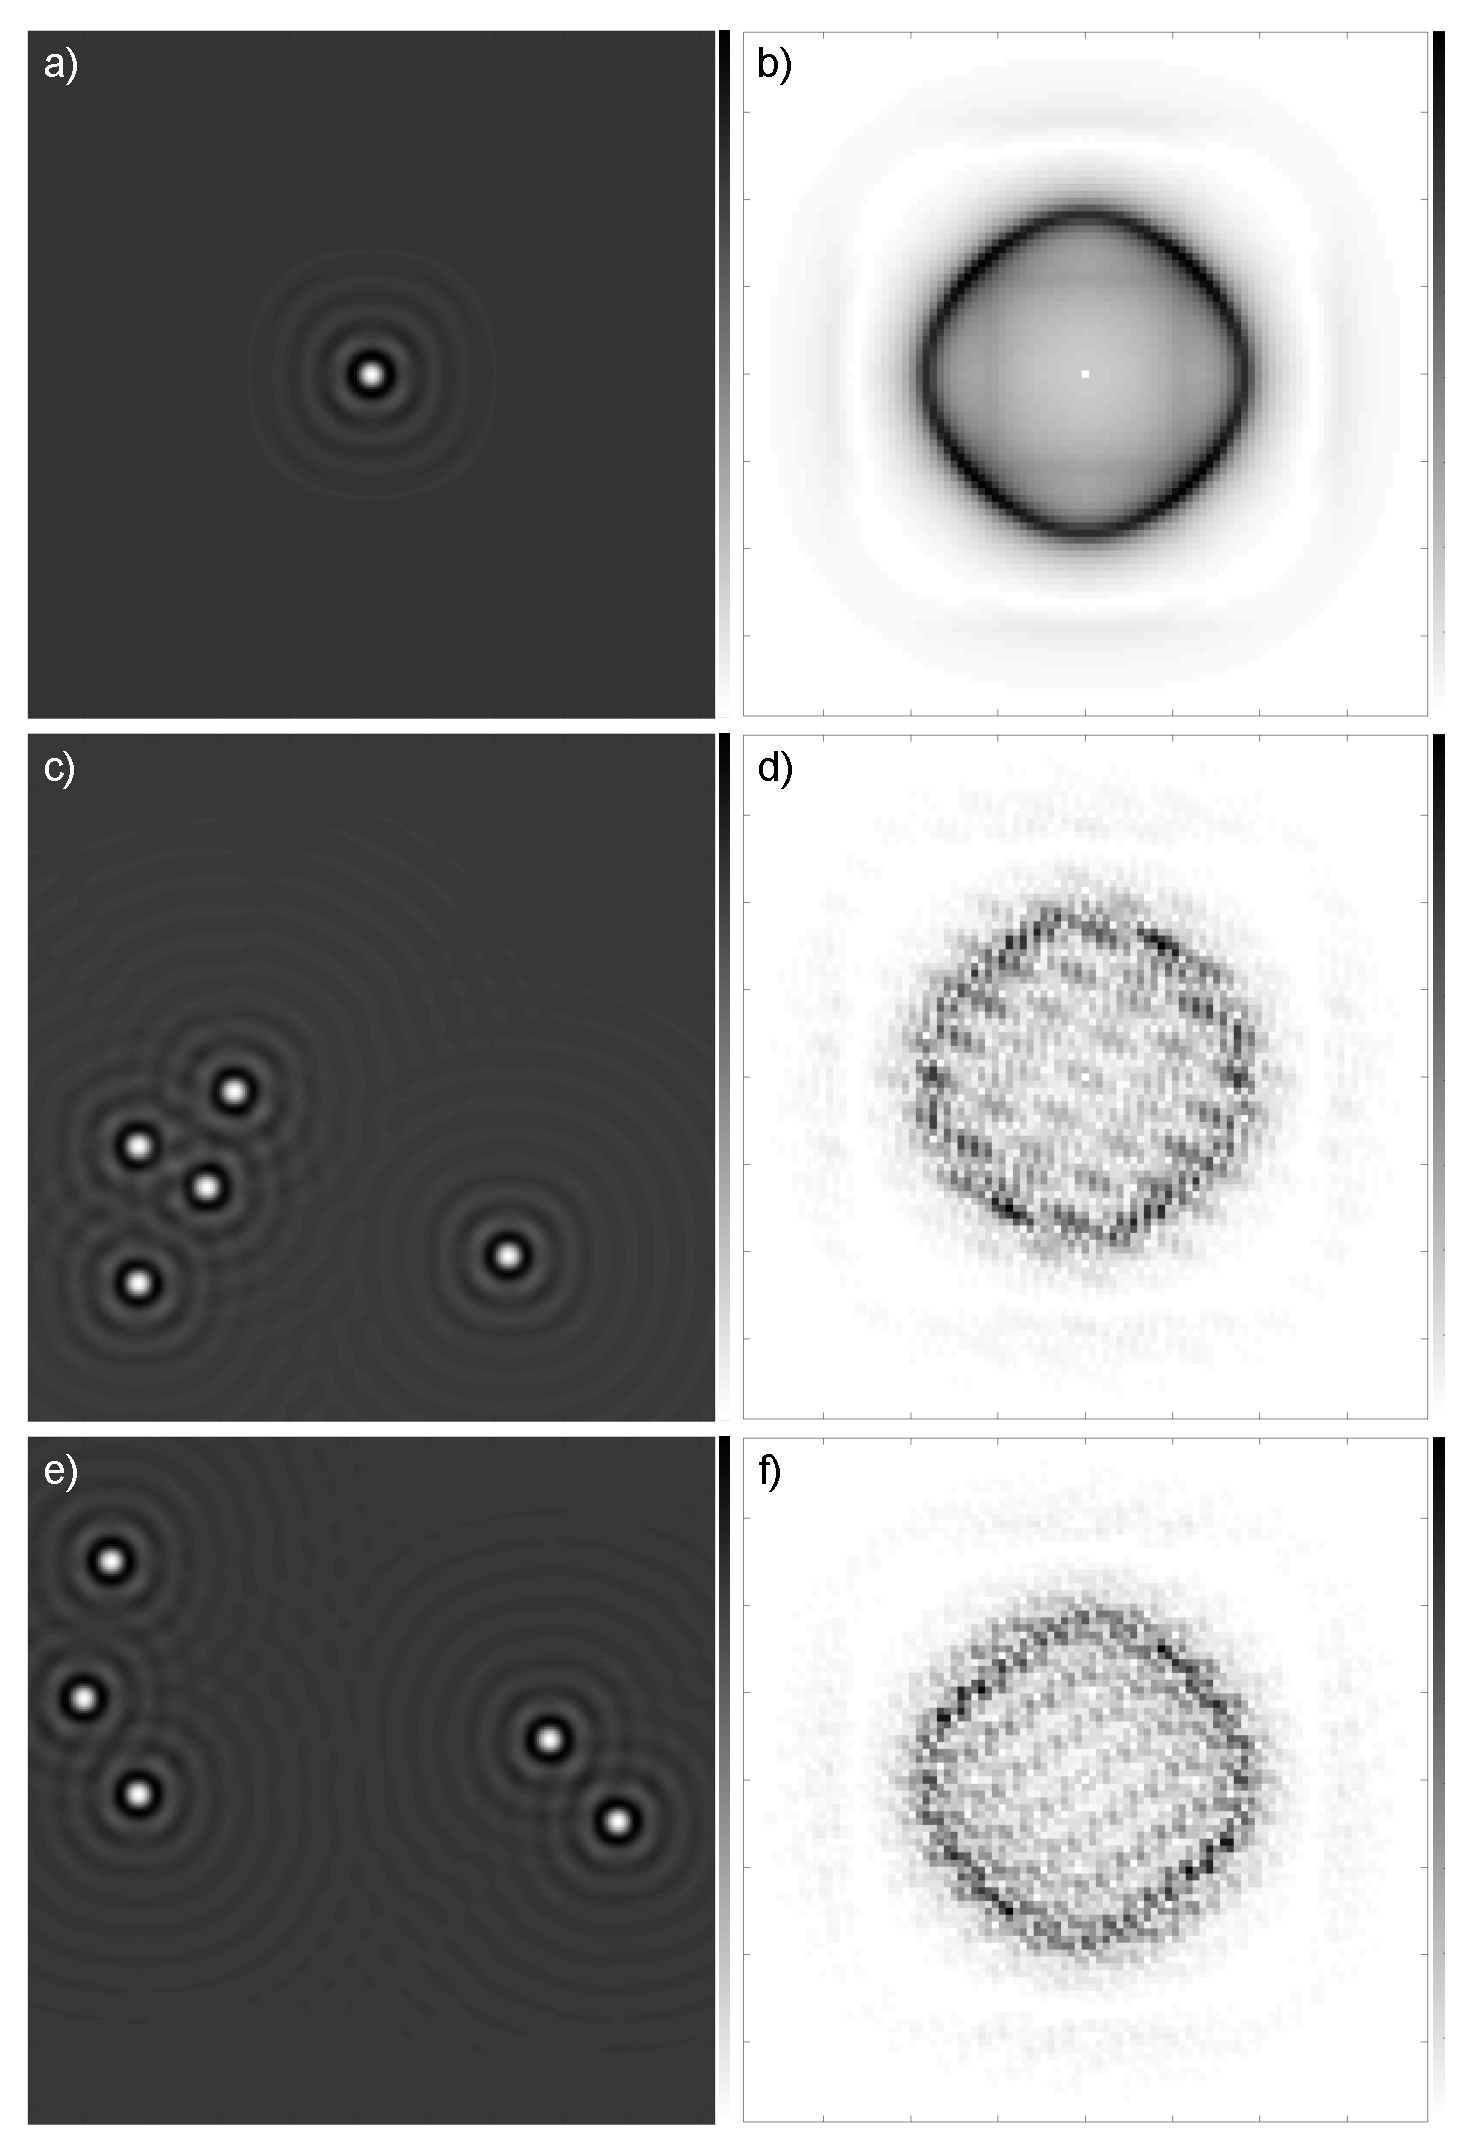
\includegraphics[width=\textwidth]{Ch5_phasenoise.pdf} 
	\centering
	\caption{}
	\label{fig:ch5_phasenoise}
\end{figure}

Beyond the phenomenological illustration, we can further understand the source of phase noise with a mathematical analysis on multi-defect $\delta\rho(\textbf{x},\omega)$. We first discuss the form of the multi-defect T-matrix T, it is a $N_d \times N_d$ square matrix with entry T$_{\alpha \beta}$ representing the cross scattering term between defect m and n. We then separate the diagonal and off-diagonal terms and express T as:
\begin{align}
	\ T_{\alpha\beta} &= t_{\alpha} \delta_{\alpha\beta} + t_{\alpha} G_{0\alpha\beta} (1 - \delta_{\alpha\beta}) t_{\beta} + \sum_{\alpha' \neq \alpha, \beta} t_{\alpha} G_{0\alpha\alpha'} t_{\alpha'} G_{0\alpha'\beta} t_{\beta} + \cdots \label{eq_tmul}\\
	&= t_{\alpha} \delta_{\alpha\beta} + t_{\alpha} \sum_{\alpha'} \check{G}_{\alpha\alpha'} \ T_{\alpha'\beta},
\end{align}
\noindent where $t_{\alpha}$ is the T-matrix of a single impurity at site $\alpha$ and expressed om a matrix form in a localized basis set (ie, expressed as the matrix with same dimension as the multi-defect case but with only the $\alpha$'s diagonal entry none empty). And matrix $\check{G}_{\alpha\alpha'} = G_{0\alpha\alpha'}(1-\delta_{\alpha\alpha'})$ 








